\begin{blocksection}
\question
%\begin{parts}

%\part

Given the circuit diagram below, inputs A, B, and C, and output D, write down the truth table.

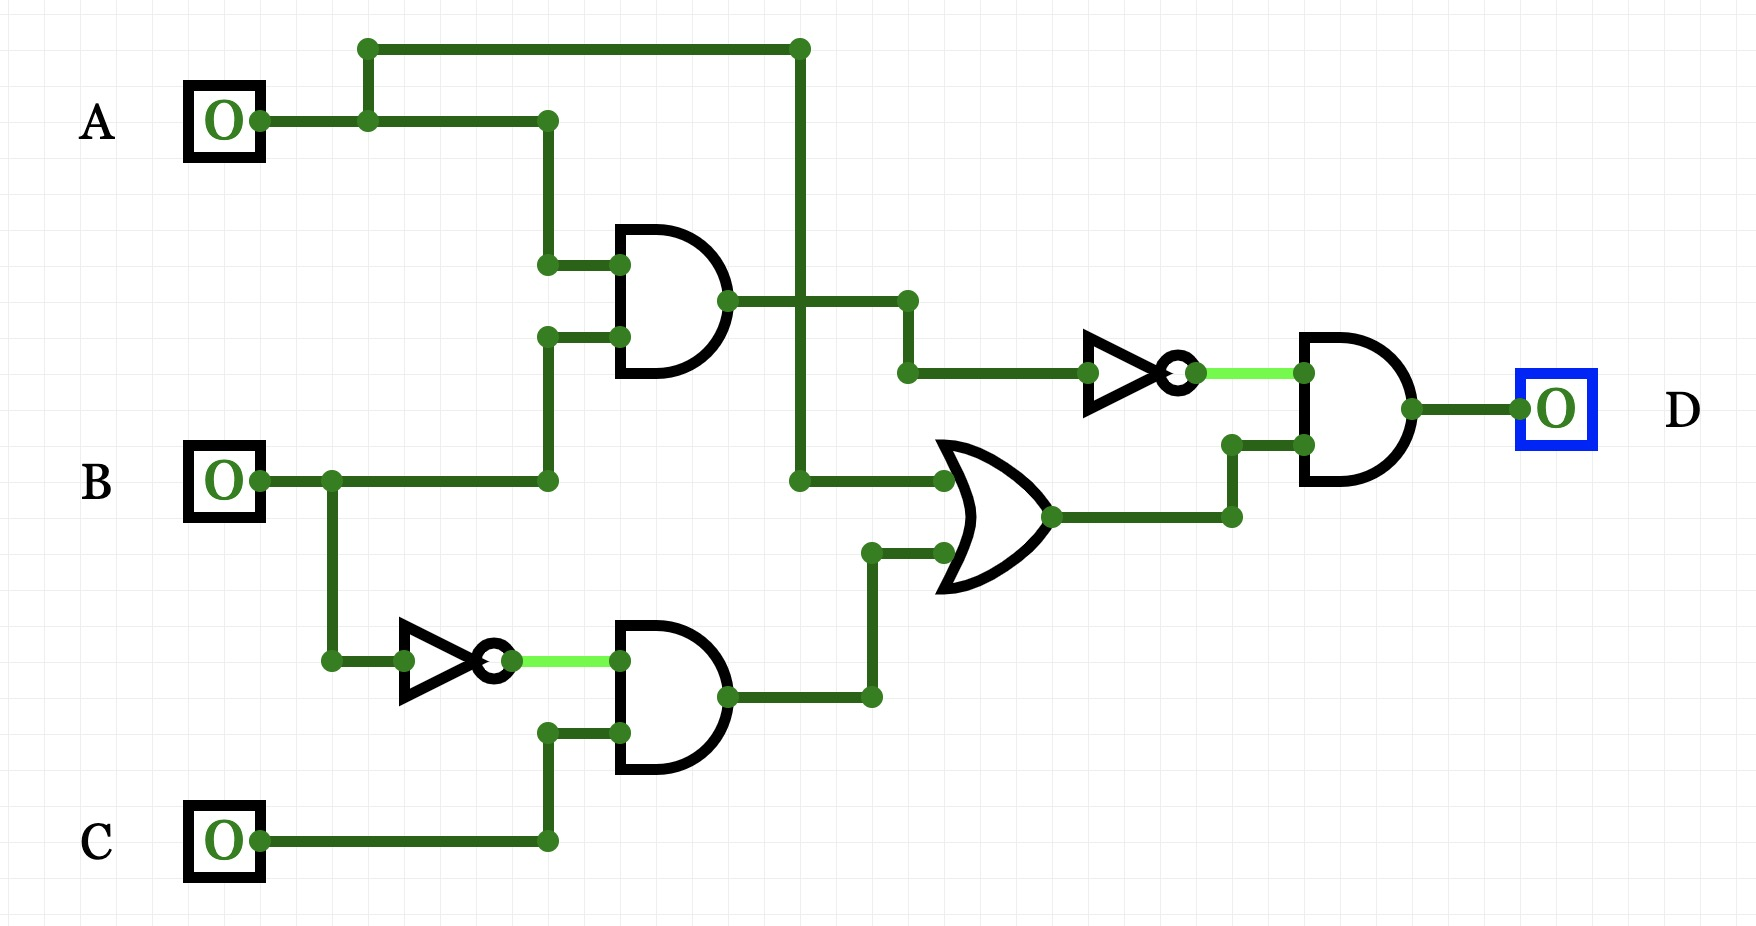
\includegraphics[width=\textwidth]{logic/boolAlgebraCircuit}

\begin{tabular}{c c c c}
A		&B		&C 		&D \\
1		&1		&1		& \\
1		&1		&0		& \\
1		&0		&1		& \\
1		&0		&0		& \\
0		&1		&1		& \\
0		&1		&0		& \\
0		&0		&1		& \\
0		&0		&0		& \\
\end{tabular}

\begin{solution}
\begin{tabular}{c c c c}
A		&B		&C 		&D \\
1		&1		&1		&0 \\
1		&1		&0		&0 \\
1		&0		&1		&1 \\
1		&0		&0		&1 \\
0		&1		&1		&0 \\
0		&1		&0		&0 \\
0		&0		&1		&1 \\
0		&0		&0		&0 \\
\end{tabular}
\end{solution}

\end{blocksection}
\begin{blocksection}

%\part
\question

Convert the truth table above to a boolean logic expression.

\begin{solution}[0.2in]
Using the Sum of Products rule:
$$A\bar{B}C + A\bar{B}\bar{C} + \bar{A}\bar{B}C$$
\end{solution}

\end{blocksection}
\begin{blocksection}

%\part
\question

Simplify the above boolean expression.
\begin{solution}[0.2in]
\begin{aligned}
$$A\bar{B}C + A\bar{B}\bar{C} + \bar{A}\bar{B}C &= \bar{B}(AC + A\bar{C} + \bar{A}C) \\
        &= \bar{B}(AC + A\bar{C} + AC + \bar{A}C) \\
        &= \bar{B}(A(C + \bar{C}) + C(A + \bar{A})) \\
        &= \bar{B}(A + C) $$
\end{aligned}
\end{solution}

\end{blocksection}
\begin{blocksection}

%\part
\question

Express the simplified boolean expression in circuit form.

\begin{solution}[0.5in]

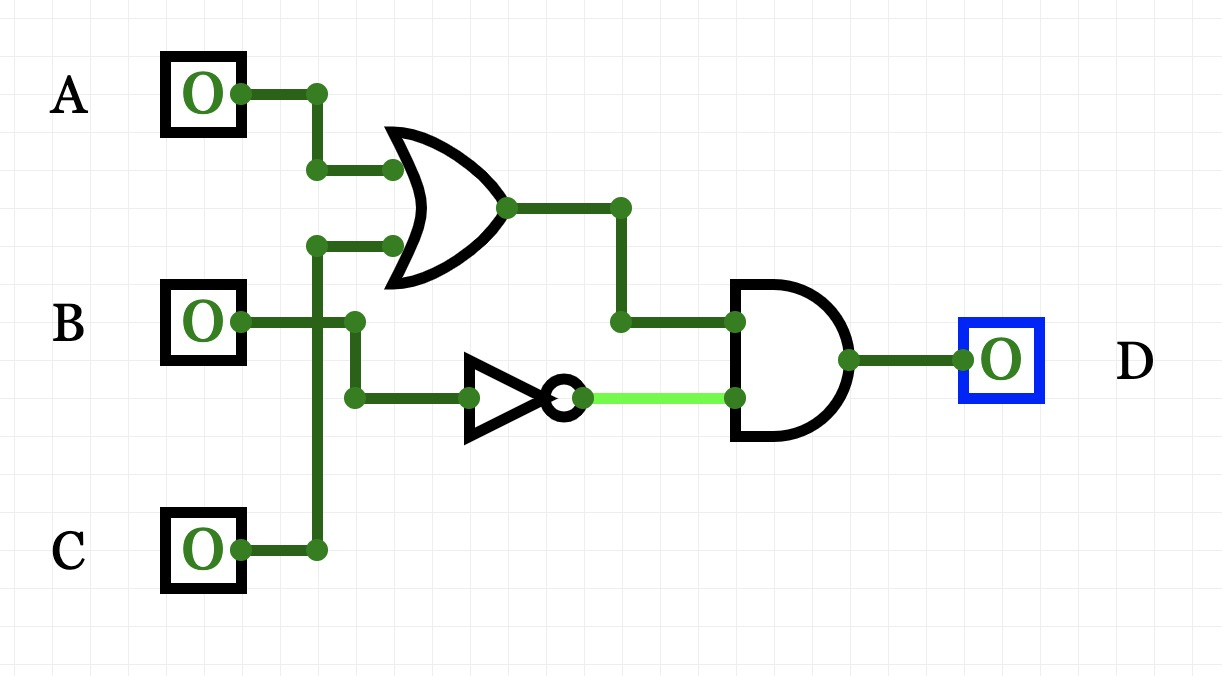
\includegraphics[width=\textwidth]{logic/boolAlgebraCircuitSol}

\end{solution}

%\end{parts}

\end{blocksection}